\section{Background}
\label{sec:hyperscanner:bkgd}
\subsection{Classic Bluetooth device discovery}
This section describes the Bluetooth scanning approach as described in the Bluetooth specification.
%
This is the process used by current protocol-compliant scanning tools such as smartphone apps.
%
Classic Bluetooth device discovery follows a time-slotted ALOHA approach.
%
The scanner sends inquiry request packets on certain frequency channels and then listens for responses in alternating $625\mu$s time slots.
%
Every request time slot, the scanner sends two inquiry (ID) requests on two different channels, switching to a different pair of channels in the next request time slot.
%
Devices hear for ID packets and then respond with inquiry response (FHS) packets that contain information that we intend to collect for device auditing (MAC address, device type and other fields).
%
Devices respond back with the FHS packets exactly 625 $\mu$s after they hear the ID packet, on the corresponding response channels.
%
\begin{figure}
    \centering
    \captionsetup{justification=centering}
    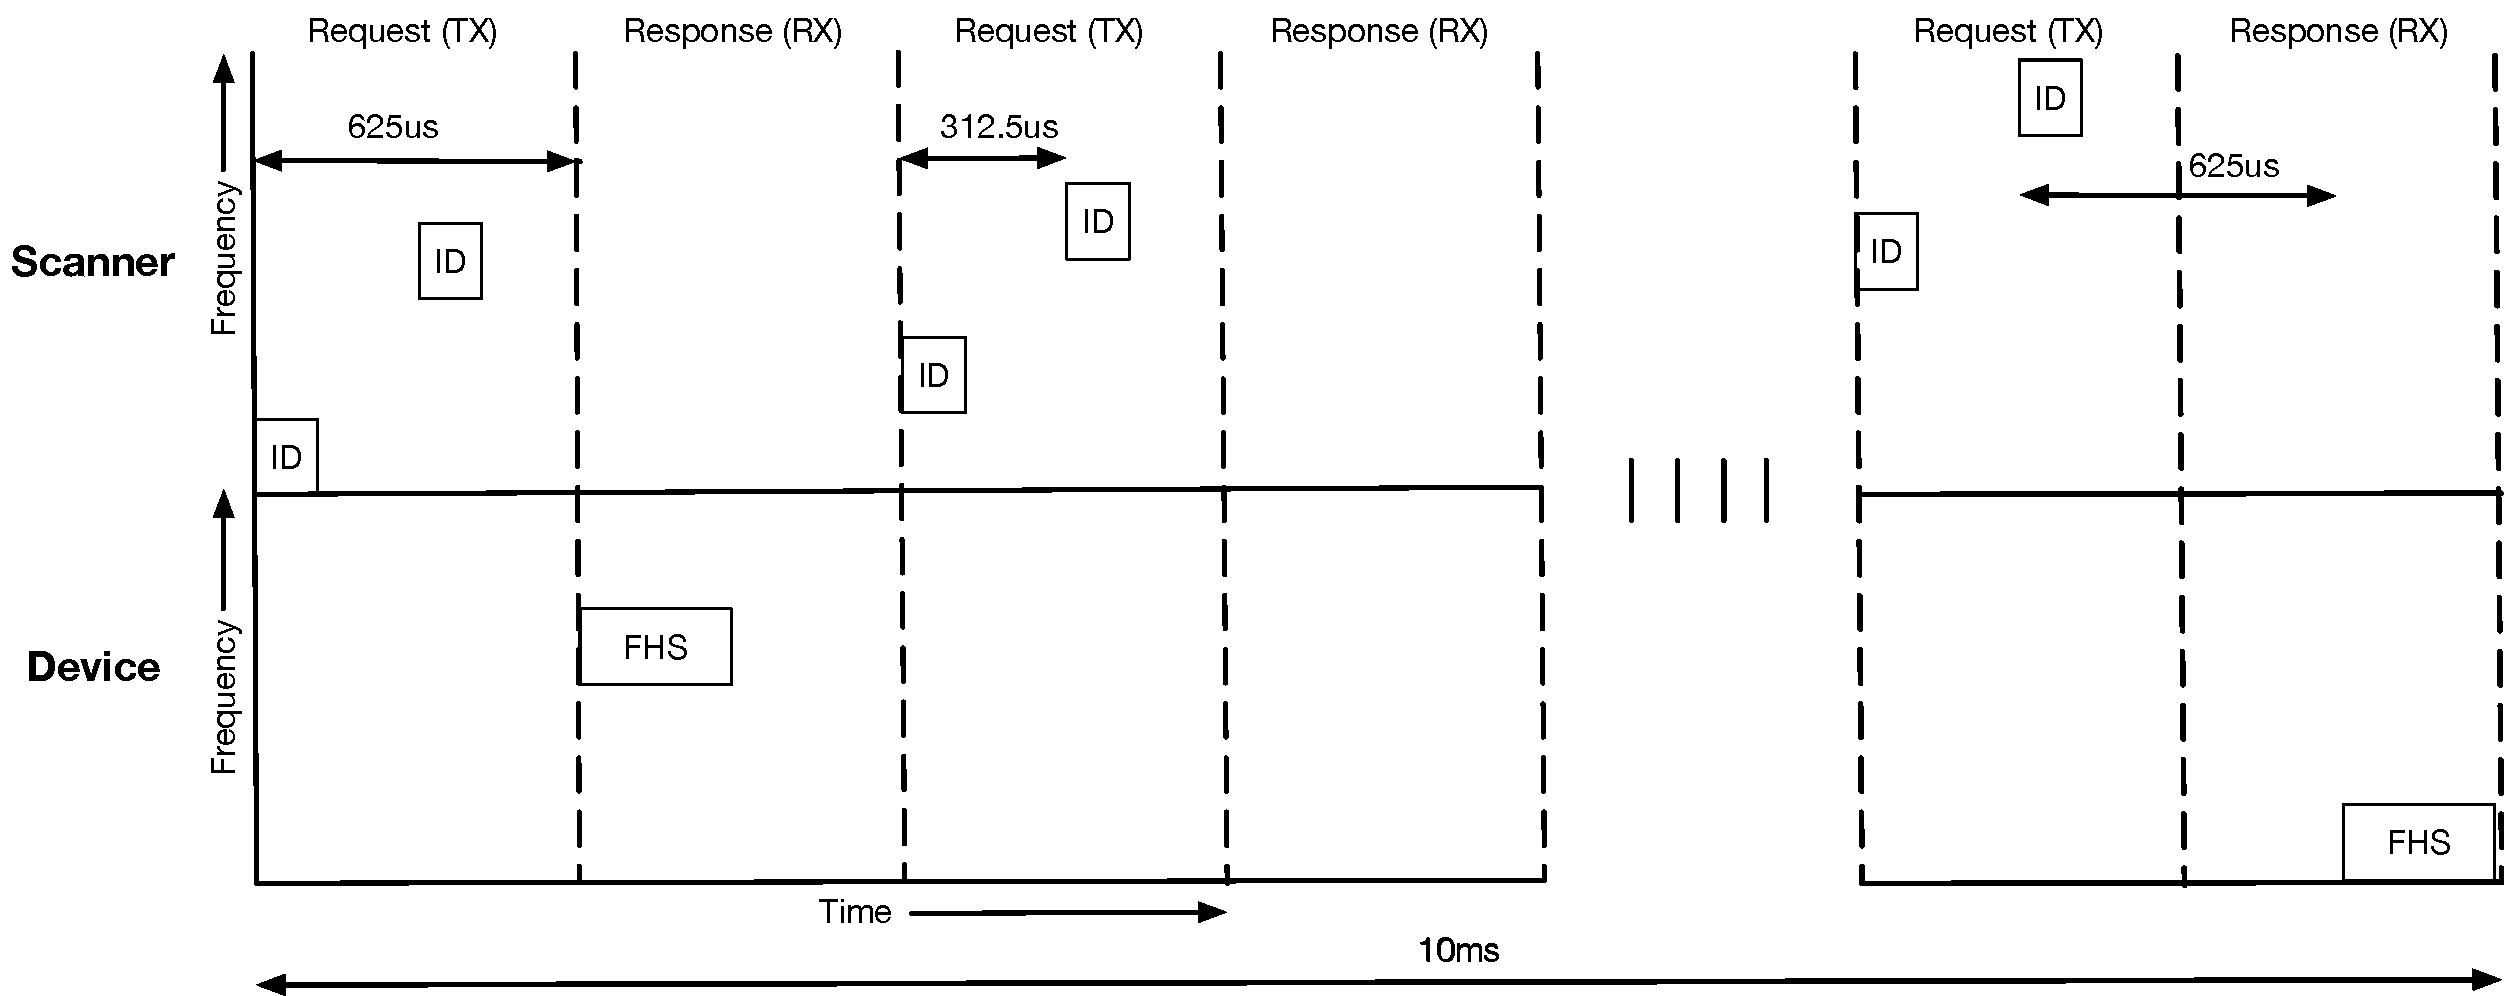
\includegraphics[width=\linewidth]{hyperscanner/figs/bt_single_chan.pdf}
    \caption{Classic Bluetooth device discovery process}
    \label{fig:hyperscanner:bt_single_chan}
\end{figure}

There are 64 non-overlapping 1 MHz channels used for discovery -- 32 request channels, and corresponding 32 response channels with a one-to-one mapping.
%
This ensures the scanner and device both know exactly which channels to receive/transmit ID/FHS packets on.
%
Figure~\ref{fig:hyperscanner:inq_resp_map} shows the mapping of request and response channels.
%
The scanner sequentially cycles through 16 of the 32 channels, sending ID packets on two channels every request time slot.
%
This full set of 16 channels comprises one inquiry train.
%
\begin{figure}
    \centering
    \captionsetup{justification=centering}
    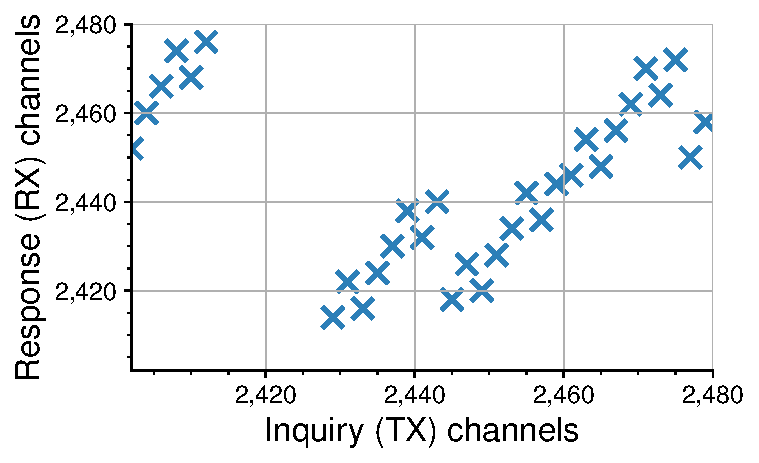
\includegraphics[width=0.6\linewidth]{hyperscanner/plots/inq_resp_map.pdf}
    \caption{Mapping of inquiry request and response frequency channels for classic Bluetooth}
    \label{fig:hyperscanner:inq_resp_map}
\end{figure}



\subsubsection*{Bluetooth scanning is slow}
The Bluetooth inquiry process was designed for low-power devices, and for avoiding interference in the 2.4 GHz band.
%
A Bluetooth device doesn't listen constantly for ID packets; a typical device will only listen for ID packets on one frequency channel for 11.25 ms in a 1.28 second interval.
%
At the end of 1.28s interval, the device switches the frequency channel in order to minimize impact of potential interference.
%
Consequently, scanners need to repeat the inquiry train several times to ensure that when a device actually wakes up it receives an ID packet.
%
In particular, scanners repeat an inquiry train of 16 channels 256 times (2.56s in total), and then move onto the other train of 16 channels.
%
In order to minimize collisions, the trains also swap one frequency member every 1.28s.
%
Consequently, the specification mentions that the inquiry process must run for at least 10.24s in a noise-free environment, and at least 40.96s in a noisy environment to guarantee we receive FHS packet from every device.
%
This scan speed is very slow, resulting in likely missed devices when driving around with a mobile scanner.


